%%%%%%%%%%%%%%%%%%%%%%%%%%%%%%%%%%%%%%%%%%%%%%%%%%%%%%%%%%%%%%%%%%%%%%%%%%%%%%%%
\chapter{ПОСТАНОВКА ЗАДАЧИ, ВЫБОР СПОСОБА РЕШЕНИЯ}
%%%%%%%%%%%%%%%%%%%%%%%%%%%%%%%%%%%%%%%%%%%%%%%%%%%%%%%%%%%%%%%%%%%%%%%%%%%%%%%%

\section{Постановка задачи}

В современном мире коммуникации через интернет становятся очень удобными, и экономят время. Такие коммуникации особенно будут экономить время, если их встроить в CRM-системы.

В связи с этим задача будет написать модуль SIP-телефона для web-браузера. Такой модуль должен быть кросс-браузерным, и иметь возможность без сложностей встраиваться в любое web-приложение, например, CRM-систему.

Обычно софт-фоны поддерживают передачу видео, аудио и мгновенных сообщений. Однако в данной работе ограничимся только передачей аудио потока.

\section{Выбор способа решения}

Для реализации данной задачи, будем использовать технологию WebRTC (см. главу \ref{chapter:analysis}). Существуют две реализации технологии WebRTC по протоколу SIP на JavaScript: библиотека sipML5 и библиотека JsSIP.\cite{sipML5}\cite{JsSIP}

Размер библиотеки JsSIP ~130kb. Размер библиотеки sipML5 чуть больше 1Mb. Однако JsSIP требует установки Node.js на сервере.

Обе библиотеки довольно неплохие и имеют следующие преимущества:
\begin{enumerate}
\item хорошая документация
\item возможность осуществления аудио и видео звонков
\item возможность отправки мгновенных сообщений
\item поддержка статуса присутствия в сети
\item функция удержания вызова
\item функция отключения микрофона
\item тональный набор (DTMF)
\end{enumerate}

Помимо этого в библиотеке sipML5 имеется функции трансляции экрана (пока что только для Google Chrome), перенаправления вызова и группового звонка.

Хоть и обе библиотеки довольно хороши, для нашей задачи выберем библиотеку sipML5, потому что функциональность у неё больше и не нужно дополнительно устанавливать Node.js на сервер.

На рисунке \ref{image:modulesStructure} под номером 4 изображён разрабатываемый модуль. У которого имеется должно быть ядро, которое выполняет функции звонков, и модули подключения к конкретной CRM-системе: Authentication, Calls, Click-to-call.

\begin{figure}[h!]
\center{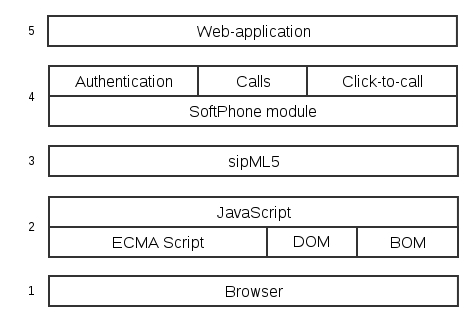
\includegraphics[width=0.75\linewidth]{modulesStructure}}
\caption{Структура взаимодействия модулей}
\label{image:modulesStructure}
\end{figure}

Ядро должно содержать код, который оборачивает библиотеку sipML5 и предоставляет функции аутентификации на сервере и звонка. Так же должно включать независимую от библиотеки часть, которая контролирует состояние сессий аутентификации и звонка.

Модуль Authentication должен выполнять запрос данных о SIP-аккаунте пользователя CRM-системы. Модуль Calls должен регистрировать звонки в CRM-системе. Модуль Click-to-call должен открывать софт-фон по клику на номер телефона, и заполнять им поле вызова.

Графический интерфейс должен состоять из скользящей кнопки и плавающего окна, которое появляется и скрывается по нажатию на эту кнопку. Плавающее окно должно включать кнопки вызова и сброса, которые меняются во время входящего звонка на кнопки снятия трубки и отклонения звонка соответственно.